\clearpage
\section{Channel6 integrator repeat after pressing the CFD board: INCOMPLETE}
The owner pressed CFD6 and confirmed DAC2/3 connected to J6 on physical6.
A fresh independent acquisition passed MCU1803, FPGA ff2f746c and power guards.
No programming, PLL change, Kasli output release or SMU access. DAC-A remained0.
The original gate mode and validation thresholds were unchanged.
The13-point coarse acquisition completed, but the controller again found no
unambiguous bank-B integration/reset template near balance. Fine and independent
return qualification did not run. A shows a sign reversal, but neither bank is
claimed to have completed the full fine/return protocol in this attempt.
\subsection{Raw comparison with the preceding attempt}
Below are unaligned raw captures at the same commanded differential offset0.
Pressing did not remove the observed ambiguity. This does not determine whether
the cause is hardware, sampling position or waveform-based phase assignment.
No particular intermittent contact or hardware defect has been established.
\begin{center}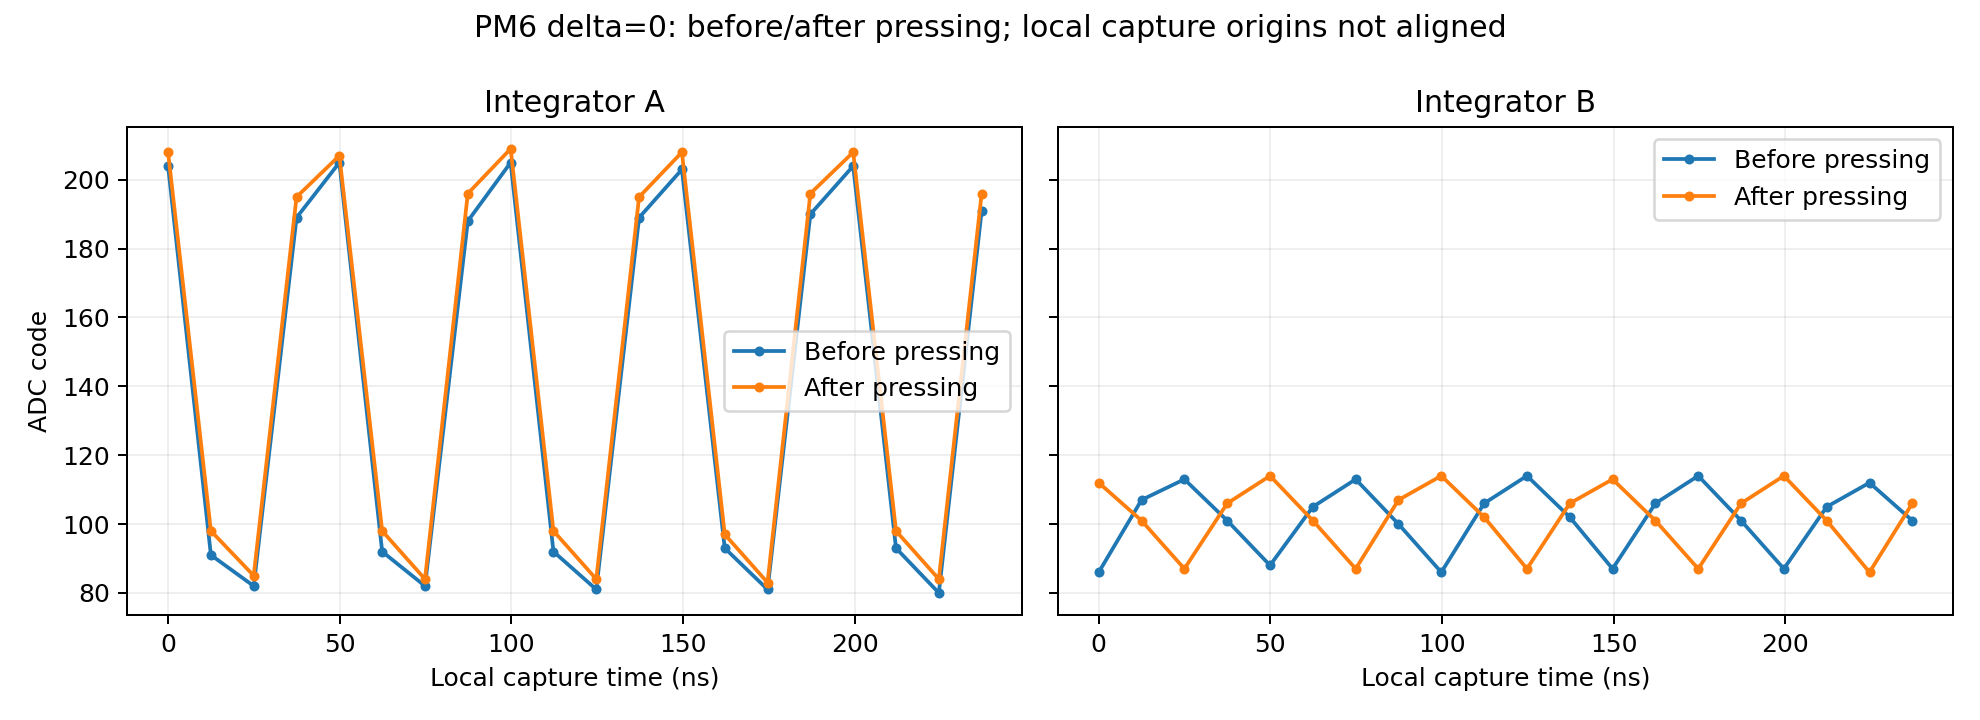
\includegraphics[width=\linewidth]{reseat06-before-after.png}\end{center}
\begin{center}\begin{tabular}{lrr}\toprule
Attempt & A mean(code) & B mean(code)\\\midrule
Before pressing & 143.530 & 102.564 \\
After pressing & 143.610 & 102.832 \\
\bottomrule\end{tabular}\end{center}
The latest INCOMPLETE repeat was explicitly selected; the original incomplete
record and phase diagnostics remain immutable. Every other selected result ID
is unchanged. ADC5--12 and integrators5,7--12 retain their previous PASS results.
Final channel6 amplifiers disabled, direct bypass isolated, monitors inhibited,
TCA masks zero. External DAC channels0/1 are1/1V, channels2/3 are1.024/2.048V.
Leases released. Source and raw-data hashes are retained with the repeat.
